\documentclass{article}
% Change "article" to "report" to get rid of page number on title page
\usepackage{amsmath,amsfonts,amsthm,amssymb}
\usepackage{setspace}
\usepackage{Tabbing}
\usepackage{fancyhdr}
\usepackage{lastpage}
\usepackage{extramarks}
\usepackage{chngpage}
\usepackage{soul,color}
\usepackage{graphicx,float,wrapfig}
\usepackage{titlesec}
\usepackage{apacite} 
\usepackage{tikz}
\usepackage{tkz-berge}
\usepackage[position=top]{subfig}
 \usepackage{parskip}
 \usepackage{listings}

% In case you need to adjust margins:
\topmargin=-0.25in      %
\evensidemargin=0.2in     %
\oddsidemargin=0.2in      %
\textwidth=6.2in        %
\textheight=9.0in       %
\headsep=0.35in         %

% Homework Specific Information
\newcommand{\hmwkTitle}{Homework\ \#1}
\newcommand{\hmwkSubTitle}{}
\newcommand{\hmwkDueDate}{Monday,\ September\ 19,\ 2016}
\newcommand{\hmwkClass}{CS\ 590-AI}
\newcommand{\hmwkClassInstructor}{Lecture: Prof. Elias Bareinboim}
\newcommand{\hmwkAuthorName}{Andreas Waldis}
                                           %

\pagestyle{fancy}                                                    %
\lhead{\hmwkAuthorName}   
\fancyhf{}
\fancyhead[L]{\lastmark}
\fancyhead[R]{\thepage}
\renewcommand{\headrulewidth}{0pt}

\pagestyle{fancy}
\fancyhf{}
\rhead{\leftmark}
\lhead{Andreas Waldis}
\cfoot{\thepage}
\renewcommand{\headrulewidth}{0.3pt}
 
% This is used to trace down (pin point) problems
% in latexing a document:
%\tracingall

%%%%%%%%%%%%%%%%%%%%%%%%%%%%%%%%%%%%%%%%%%%%%%%%%%%%%%%%%%%%%
% Some tools
\newcommand{\enterProblemHeader}[1]{\nobreak\extramarks{#1}{#1 continued on next page\ldots}\nobreak%
                                    \nobreak\extramarks{#1 (continued)}{#1 continued on next page\ldots}\nobreak}%
\newcommand{\exitProblemHeader}[1]{\nobreak\extramarks{#1 (continued)}{#1 continued on next page\ldots}\nobreak%
                                   \nobreak\extramarks{#1}{}\nobreak}%

\newlength{\labelLength}
\newcommand{\labelClue}[2]
  {\settowidth{\labelLength}{#1}%
   \addtolength{\labelLength}{0.25in}%
   \changetext{}{-\labelLength}{}{}{}%
   \noindent\fbox{\begin{minipage}[c]{\columnwidth}#2\end{minipage}}%
   \marginpar{\fbox{#1}}%

   % We put the blank space above in order to make sure this
   % \marginpar gets correctly placed.
   \changetext{}{+\labelLength}{}{}{}}%

\setcounter{secnumdepth}{0}
\newcommand{\homeworkProblemName}{}%
\newcounter{homeworkProblemCounter}%
\newenvironment{homeworkProblem}[1][Problem \arabic{homeworkProblemCounter}]%
  {\stepcounter{homeworkProblemCounter}%
   \renewcommand{\homeworkProblemName}{#1}%
   \section{\homeworkProblemName}%
   \enterProblemHeader{\homeworkProblemName}}%
  {\exitProblemHeader{\homeworkProblemName}}%

\newcommand{\problemClue}[1]
  {\noindent\fbox{\begin{minipage}[c]{\columnwidth}#1\end{minipage}}}%

\newcommand{\problemLClue}[1]
  {\labelClue{\homeworkProblemName}{#1}}

\newcommand{\homeworkSectionName}{}%
\newlength{\homeworkSectionLabelLength}{}%
\newenvironment{homeworkSection}[1]%
  {% We put this space here to make sure we're not connected to the above.
   % Otherwise the changetext can do funny things to the other margin

   \renewcommand{\homeworkSectionName}{#1}%
   \settowidth{\homeworkSectionLabelLength}{\homeworkSectionName}%
   \addtolength{\homeworkSectionLabelLength}{0.25in}%
   \changetext{}{-\homeworkSectionLabelLength}{}{}{}%
   \subsection{\homeworkSectionName}%
   \enterProblemHeader{\homeworkProblemName\ [\homeworkSectionName]}}%
  {\enterProblemHeader{\homeworkProblemName}%

   % We put the blank space above in order to make sure this margin
   % change doesn't happen too soon (otherwise \sectionClue's can
   % get ugly about their \marginpar placement.
   \changetext{}{+\homeworkSectionLabelLength}{}{}{}}%

\newcommand{\sectionClue}[1]
  {% We put this space here to make sure we're disconnected from the previous
   % passage

   \noindent\fbox{\begin{minipage}[c]{\columnwidth}#1\end{minipage}}%
   \enterProblemHeader{\homeworkProblemName}\exitProblemHeader{\homeworkProblemName}%
   \marginpar{\fbox{\homeworkSectionName}}%

   % We put the blank space above in order to make sure this
   % \marginpar gets correctly placed.
   }%

%%%%%%%%%%%%%%%%%%%%%%%%%%%%%%%%%%%%%%%%%%%%%%%%%%%%%%%%%%%%%


%%%%%%%%%%%%%%%%%%%%%%%%%%%%%%%%%%%%%%%%%%%%%%%%%%%%%%%%%%%%%
% Make title
\title{\vspace{2in}\textmd{\textbf{\hmwkClass,\ \hmwkTitle \textit{\\\hmwkSubTitle}}}\\\normalsize\vspace{0.1in}\small{Due\ on\ \hmwkDueDate}\\\vspace{0.1in}\large{\textit{\hmwkClassInstructor\ }}\vspace{3in}}
\date{}
\author{\textbf{\hmwkAuthorName}}
%%%%%%%%%%%%%%%%%%%%%%%%%%%%%%%%%%%%%%%%%%%%%%%%%%%%%%%%%%%%%

\begin{document}
\begin{spacing}{1.2}
\pagenumbering{Roman}
\maketitle
\newpage
% Uncomment the \tableofcontents and \newpage lines to get a Contents page
% Uncomment the \setcounter line as well if you do NOT want subsections
%       listed in Contents
%\setcounter{tocdepth}{1}
\tableofcontents

\newpage 
% When problems are long, it may be desirable to put a \newpage or a
% \clearpage before each homeworkProblem environment

\pagenumbering{arabic}
\section{Exercise \#1 - Search Algorithmus}

\begin{center}
 \begin{tabular}{|c|c|c|c|c|} 
 \hline
 (a) BFS  & (b) DFS & (c) UCS & (d) Greedy  & (e) A*\\ [1ex] 
 \hline\hline
 LWSN & LWSN & LWSN & LWSN & LWSN \\ 
 \hline
 ELLT & ELLT & ELLT & ELLT & ELLT \\ 
 \hline
 HAAS & WTHR & HAAS & WTHR & WTHR \\ 
 \hline
 BRNG & HEAV & SC & HEAV & HEAV \\ 
 \hline
 WTHR & \textbf{PMU} & WTHR & \textbf{PMU} & HAAS \\ 
 \hline
 HEAV &   & HEAV &  &  \textbf{PMU} \\ 
 \hline
 UNIV &  & BRNG &  &  \\ 
 \hline
 REC &   & REC &  &  \\ 
 \hline
 STEW &   &  \textbf{PMU} &  &  \\ 
 \hline
 \textbf{PMU} &  &  &  &  \\ 
 \hline
\end{tabular}
\end{center}

\section{Exercise \#2 - Search and Heuristics}


\subsection{(a) - DFS vs. BFS }

\textbf{Explain when DFS is better than BFS and vice-versa.}
\begin{center}
$b$ as branching factor\\
$d$ as depth of the solution\\
$h$ as height of the tree, $d<h$\\
DFS takes $O(b^h)$ with $O(h*m)$ space\\
BFS takes $O(b^d)$ with $O(b^h)$ space\\
\end{center}

Based on the complexities for time and space, DFS a better algorithmus for the following cases

\begin{itemize}
\item There is a limited amount of space available, because DFS needs $max$ $height * branching$ $factor$ space ($O(h*m)$)
\item If the size of $\Delta$level between root and solution does not matter
\item When it is necessary to detect loops in the graph
\end{itemize}

On the other hand, BFS is to prefere for the following situations, 
\begin{itemize}
\item If solution is near to the root,  $\Delta$level between root and solution is small
\item The shortest path information (fewest edges) is needed, because all edges are stored
\end{itemize}

\subsection{(b) - Heuristic}

\textbf{Explain why, in heuristic search, it is a good idea to underestimate the cost value until the goal
instead of overestimating it.}\\
Because if the heuristic function is overestimating it wont be a admissible heuristic anymore, because $h(n)\leq h'(n)$ 

\subsection{(c) - Lack of consistency }

\textbf{Explain how and why the lack of consistency can lead to some problems with graph heuristic
search? You can give an example, but also need to provide a clear and logical explanation with
words.}

Consistency is defined as $h(n) \leq c(n,n') + h(n')$ which means that the heuristic function of the node $n$ can not be bigger than the sum of the cost to get from node $n$ to $n'$ and the heuristic function of node $B$. If this is not the case its possible to loose a optimal solution and the whole search is not optimal anymore. 

\subsection{(d) - Lack of consistency }

\textbf{Prove that consistency implies admissibility.}\\
Assume that there are three nodes $A, B, G$, $G = goal$, $A, B \in closest path$, the definition of admissibility  $h(n)\leq h'(n)$  and consistency ($h(n) \leq c(n,n') + h(n')$).
\begin{itemize}
\item Base case, when there are 0 steps from the current node to the goal node, it applies that $h(n) = h(G) = 0 \leq h'(G)$.
\item Induction step, there is a closest path to goal node including the following sequence $...,A,B,...,G$ and $h(A) \leq h'(A)$, $h(A) \leq c(A,B) + h(B)$ and $h(B) \leq h'(B)$. Thus $h(A) \leq c(A,B) + h'(B) = h'(A)$, because $c(A,B)$ is the actual cost between $A$ and $B$ and $h'(B)$ is the actual cost from $B$ to $G$ to sum of both must be the actual cost from $A$ to $G$.
\end{itemize}

\subsection{(e) - Optimality of A* }

\textbf{Prove that A* is optimal in graph search if the heuristic is consistent.}\\
Consider the fact, that a consistence graph-search can be shown as a search-tree. Which is optimal, based on the proof of optimality for the tree-search algorithms. 

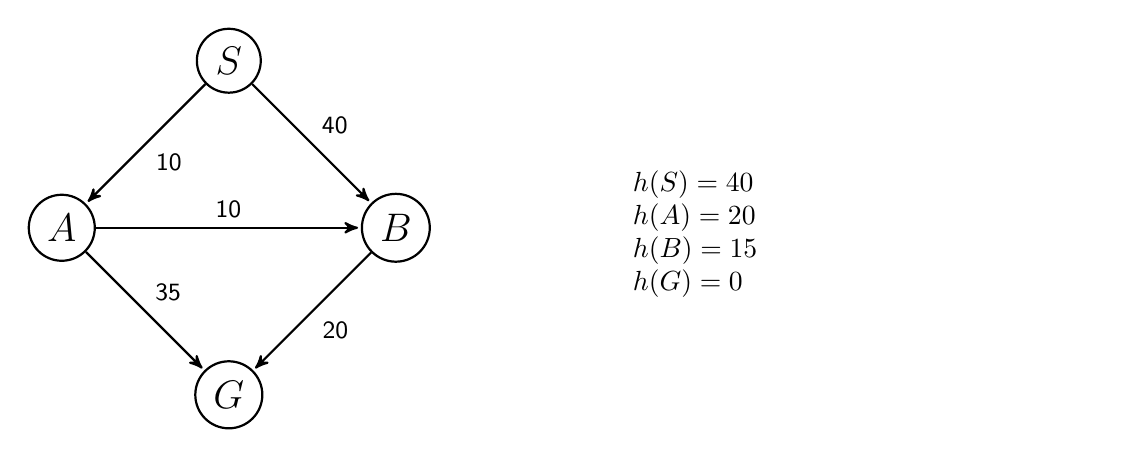
\begin{tikzpicture}[->,>=stealth',shorten >=1pt,auto,node distance=3cm,
                    thick,main node/.style={circle,draw,font=\sffamily\Large\bfseries}]

  \node[main node] (S) {$S$};
  \node[main node] (A) [below left of=S] {$A$};
  \node[main node] (B) [below right of=S] {$B$};
  \node[main node] (G) [below right of=A] {$G$};
  \node[text width=6cm, anchor=west, right] at (5,-2.2)
    {
        $h(S)=40$\\
        $h(A)=20$\\
        $h(B)=15$\\
        $h(G)=0$\\
    };

  \path[every node/.style={font=\sffamily\small}]
    (S) edge node {10} (A)
        edge node {40} (B)
    (A) edge node {35} (G)
        edge node {10} (B)
    (B) edge node {20} (G);
\end{tikzpicture}

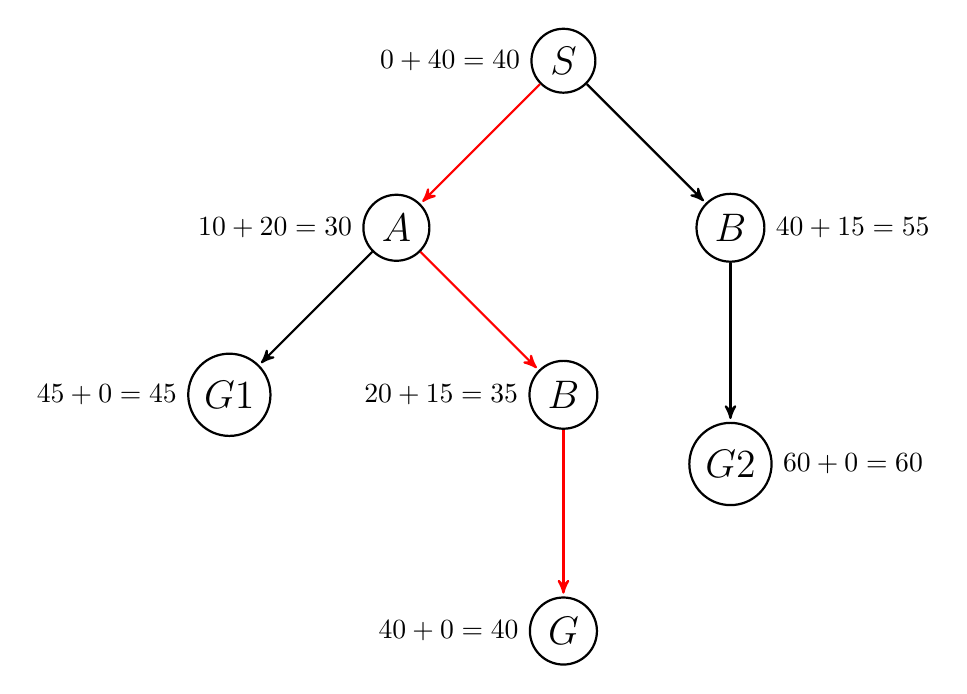
\begin{tikzpicture}[->,>=stealth',shorten >=1pt,auto,node distance=3cm,
                    thick,main node/.style={circle,draw,font=\sffamily\Large\bfseries}]

  \node[main node] (S) {$S$};
  \node[left] at (S.west) {$0+40 = 40$};
  \node[main node] (A) [below left of=S] {$A$};
  \node[left] at (A.west) {$10+20 = 30$};
  \node[main node] (B) [below right of=S] {$B$};
  \node[right] at (B.east) {$40+15 = 55$};
  \node[main node] (G1) [below left of=A] {$G1$};
  \node[left] at (G1.west) {$45+0 = 45$};
  \node[main node] (G2) [below of=B] {$G2$};
  \node[right] at (G2.east) {$60+0 = 60$};
  \node[main node] (B') [below right of=A] {$B$};
  \node[left] at (B'.west) {$20+15 = 35$};
  \node[main node] (G) [below of=B'] {$G$};
  \node[left] at (G.west) {$40+0 = 40$};

  \path[every node/.style={font=\sffamily\small}]
    (S) edge[red] node {} (A)
        edge node {} (B)
    (A) edge[red] node {} (B')
         edge node {} (G1)
    (B) edge node {} (G2)
    (B') edge[red] node {} (G);
\end{tikzpicture}

\section{Exercise \#3 - CSP}

\subsection{(a) - Variables domains \& constraints }
\textbf{State the problem as a CSP using one variable per planet. Specify the variable domains and
constraints formally.}
\textbf{Variables}, $V=\alpha, \beta, \gamma, \omega, \mu, \zeta$\\
\textbf{Diplomats}, $D={X,Y,Z}$\\
$\textbf{X}\in {\alpha, \gamma, \zeta}$\\
$\textbf{Y}\in {\alpha, \beta, \zeta, \omega, \mu}$\\
$\textbf{Z}\in {\alpha, \gamma, \omega, \mu}$\\
\textbf{Constraints}, $\alpha \neq \beta \neq \omega, \zeta \neq \omega, \mu \neq \gamma$

\subsection{(b) - Constraint graph}
\textbf{Show the constraint graph associated with your formulation.
}

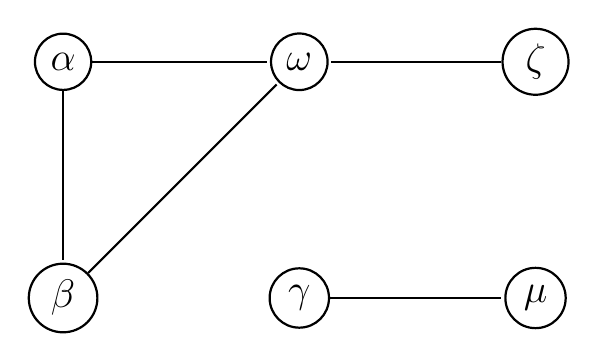
\begin{tikzpicture}[->,>=stealth',shorten >=1pt,auto,node distance=3cm,
                    thick,main node/.style={circle,draw,font=\sffamily\Large\bfseries}]

  \node[main node] (alpha) {$\alpha$};
  \node[main node] (beta) [below of=alpha] {$\beta$};
  \node[main node] (gamma) [right of=beta] {$\gamma$};
  \node[main node] (omega) [right of=alpha] {$\omega$};
  \node[main node] (mu) [right of=gamma] {$\mu$};
  \node[main node] (zeta) [right of=omega] {$\zeta$};
  
  
    \path [-] (alpha) edge node {} (beta);
    \path [-] (alpha) edge node {} (omega);
    \path [-] (beta) edge node {} (omega);
    \path [-] (gamma) edge node {} (mu);
    \path [-] (zeta) edge node {} (omega);
    
\end{tikzpicture}
\subsection{(c) - Structur}
\textbf{Does the graph have particular structure? Explain how to solve the problem in an efficient way.}
There is a independent sub problem ($\mu , \gamma$) and a nearly tree search problem. For the independent problem, we just can assign two diplomats, who are able to speech in the certain language. Next, for the nearly tree search problem we try to get a tree structure. To do this we cut out $\alpha$ and assign a possible value such as $X$.

\begin{tikzpicture}[->,>=stealth',shorten >=1pt,auto,node distance=3cm,
                    thick,main node/.style={circle,draw,font=\sffamily\Large\bfseries}]

  \node[main node] (alpha) {$\alpha$};
  \node[main node] (beta) [below of=alpha] {$\beta$};
  \node[main node] (omega) [right of=alpha] {$\omega$};
  \node[main node] (zeta) [right of=omega] {$\zeta$};
  \node[main node] (mu) [right of=gamma] {$\mu$};
  \node[main node] (gamma) [right of=beta] {$\gamma$};
  \node[left] at (alpha.west) {$X$};
  \node[left] at (gamma.west) {$Z$};
  \node[right] at (mu.east) {$Y$};
  
    \path [-] (beta) edge node {} (omega);
    \path [-] (zeta) edge node {} (omega);
    \path [-] (gamma) edge node {} (mu);
    
\end{tikzpicture}

Now we come to tree structure, where easily can assign the possible value. Of course there a lot different solution based on the first chosen diplomats.

\begin{tikzpicture}[->,>=stealth',shorten >=1pt,auto,node distance=3cm,
                    thick,main node/.style={circle,draw,font=\sffamily\Large\bfseries}]

  \node[main node] (alpha) {$\alpha$};
  \node[main node] (beta) [below of=alpha] {$\beta$};
  \node[main node] (omega) [right of=alpha] {$\omega$};
  \node[main node] (zeta) [right of=omega] {$\zeta$};
  \node[main node] (mu) [right of=gamma] {$\mu$};
  \node[main node] (gamma) [right of=beta] {$\gamma$};
  \node[left] at (alpha.west) {$X$};
  \node[left] at (gamma.west) {$Z$};
  \node[right] at (mu.east) {$Y$};
  \node[left] at (beta.west) {$Y$};
  \node[above] at (omega.north) {$Z$};
  \node[right] at (zeta.east) {$X$};
  
    \path [-] (alpha) edge node {} (beta);
    \path [-] (alpha) edge node {} (omega);
    \path [-] (beta) edge node {} (omega);
    \path [-] (gamma) edge node {} (mu);
    \path [-] (zeta) edge node {} (omega);
    
\end{tikzpicture}

\section{Exercise \#4 - Arc Consistency}

\subsection{(a) - Constraints}
\textbf{State the constraints for this problem (implicitly or explicitly).}\\
${C}_{2}\neq {C}_{3} \neq {C}_{4} {C}_{4} \neq {C}_{5}, {C}_{1} \neq {C}_{6}, {C}_{1} \neq {C}_{7}$\\
\textbf{${R}_{A}$} $\in$ ${C}_{1}, {C}_{4}, {C}_{5}, {C}_{6}$\\
\textbf{${R}_{B}$} $\in$ ${C}_{1}, {C}_{2}, {C}_{3}, {C}_{6}, {C}_{7}$\\
\textbf{${R}_{C}$} $\in$ ${C}_{2}, {C}_{3}, {C}_{5}, {C}_{7}$\\

\subsection{(b) - Arc consistency}
\textbf{Show the variable domains after enforcing arc consistency.}\\

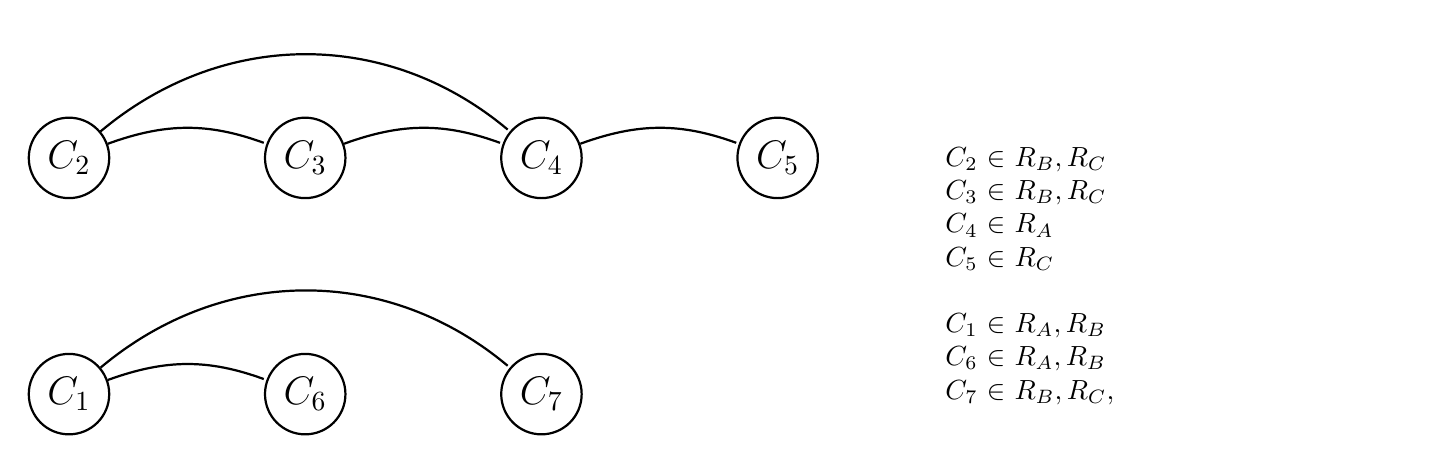
\begin{tikzpicture}[->,>=stealth',shorten >=1pt,auto,node distance=3cm,
                    thick,main node/.style={circle,draw,font=\sffamily\Large\bfseries}]

  \node[main node] (c2)  {${C}_{2}$};
  \node[main node] (c1) [below of=c2] {${C}_{1}$};
  \node[main node] (c3) [right of=c2] {${C}_{3}$};
  \node[main node] (c4) [right of=c3] {${C}_{4}$};
  \node[main node] (c5) [right of=c4] {${C}_{5}$};
  \node[main node] (c6) [right of=c1] {${C}_{6}$};
  \node[main node] (c7) [right of=c6] {${C}_{7}$};
  
  
  \node[text width=6cm, anchor=west, right] (TextNode2) at (11,-1.5)
    {
    ${C}_{2}$ $\in$ ${R}_{B}, {R}_{C}$\\
    ${C}_{3}$ $\in$ ${R}_{B}, {R}_{C}$\\
    ${C}_{4}$ $\in$ ${R}_{A}$\\
    ${C}_{5}$ $\in$ ${R}_{C}$\\~\\
    ${C}_{1}$ $\in$ ${R}_{A}, {R}_{B}$\\
    ${C}_{6}$ $\in$ ${R}_{A}, {R}_{B}$\\
    ${C}_{7}$ $\in$ ${R}_{B}, {R}_{C}$,\\
    };

    \path [-] (c2) edge[bend left=20] node {} (c3);
    \path [-] (c2) edge[bend left=40] node {} (c4);
    \path [-] (c3) edge[bend left=20] node {} (c4);
    \path [-] (c4) edge[bend left=20] node {} (c5);
    \path [-] (c1) edge[bend left=20] node {} (c6);
    \path [-] (c1) edge[bend left=40] node {} (c7);
  
    
\end{tikzpicture}

\subsection{(c) - Least constrained value ordering}
\textbf{What variables or variables should be assigned first if we use least constrained value ordering?}\\
For the first independent sub problem it doesn't matter, either ${C}_{2} -> {R}_{B}$ and  ${C}_{3} -> {R}_{C}$ or vice versa. Neither the one or the other gives us more flexibility. But in the second sub problem, ${C}_{7}$ should be assigned ${R}_{C}$, thus we have on ${C}_{1}$ and ${C}_{6}$ two possible options (${R}_{A}, {R}_{B}$).


\section{Exercise \#5 - Local search}
The basic idea is it to generate all possible results for the first row. With the given nonogram example it would be just {$(1,0,1,1,1)$} because there is no other combination possible. For example with {$(2,1)$} it would be {$(1,1,0,1,0),(1,1,0,0,1),(0,1,1,0,1)$}. In the next step each possible row will combined with possible column combination. The following matrix is a example for such a combination. \\\\
$\begin{bmatrix}
    1 & 0 & 1 & 1 & 1\\
    0 & 0 & 0 & 1 & 1\\
    1 & 0 & 0 & 1 & 0\\
    1 & 0 & 0 & 0 & 0\\
    1 & 0 & 0 & 0 & 0
\end{bmatrix}$\\

Based on this possible solution the resulting row-sets will be calculated and compared with the given the set. This comparison will end in the value, which represent the correctness of this solution. If it is equal to zero, a solution was found. Otherwise the search will continue.  

\subsection{bonus}
I implemented the algorithms with Scala, like described above. For testing I used a 5x5, 7x7 and 12x12 nonogramm. While I found a solution for the 5x5 and 7x7 nonogram, I was unable find a solution for the 12x12 nonogram. I assume, for the worst case, a complexity of $O(n!)$. Because for the 5x5 and the 7x7 I get a quick solution, but for 12x12 was not able to finish the algorithms within two hours.
\newpage

\begin{lstlisting}
val rows: List[List[Int]] = List(
    List(1,1),
    List(1),
    List(2,2),
    List(1,3),
    List(3)
  )

val cols: List[List[Int]] =  List(
    List(1,3),
    List(1,1),
    List(2),
    List(2),
    List(4)
  )
\end{lstlisting}

\begin{lstlisting}
val rows: List[List[Int]] = List(
    List(4),
    List(2,2,1),
    List(3,2),
    List(4,2),
    List(1,2),
    List(3,3),
    List(1,1,2)
  )

val cols: List[List[Int]] =  List(
    List(6),
    List(4,1),
    List(1,5),
    List(2,2),
    List(2,2),
    List(2,2),
    List(3,1)
  )
\end{lstlisting}\newpage
\begin{lstlisting}
val rows: List[List[Int]] = List(
    List(1,4,1,2),
    List(5,1,2,1),
    List(4,2,4),
    List(2,2,2,2),
    List(2,3,2),
    List(1,4,3),
    List(2,3,1,2),
    List(3,1),
    List(3,2,2),
    List(1,1,2,3),
    List(3,3),
    List(1,6,2)
  )


val cols: List[List[Int]] =  List(
    List(4,1,1,1),
    List(8),
    List(3,1,4,1),
    List(4,1,1,2),
    List(2,1,2,3),
    List(1,1,2,3),
    List(6,1,1),
    List(2,1,2),
    List(3,3,1),
    List(3,1,5),
    List(1,5,2,1),
    List(3,1,1,1)
  )
 \end{lstlisting}

\end{spacing}


\end{document}
